\documentclass{article}
\usepackage{siunitx}
%% Language and font encodings
\usepackage[english]{babel}
\usepackage[utf8x]{inputenc}
\usepackage[T1]{fontenc}
\usepackage{longtable}
\usepackage{multirow}

%% Sets page size and margins
\usepackage[a4paper,top=3cm,bottom=2cm,left=3cm,right=3cm,marginparwidth=1.75cm]{geometry}

%% Useful packages
\usepackage{amsmath}
\usepackage{graphicx,float}
\usepackage[colorinlistoftodos]{todonotes}
\usepackage[colorlinks=true, allcolors=blue]{hyperref}

\title{CSP334: Computer Networks \linebreak
Lab Assignment No 3 \linebreak
Assignment on Linux Networking Traceroute Ping Commands}
\author{Abhishek Gupta  2016UCS0012}

\begin{document}
\maketitle


\section{Q1: Traceroute Working}

\subsection{if there was no TTL field}
The TTL gets decreased by 1 whenever it encountes a hop . If there was no TTL field in traceroute at all then packet will roam around in the network infinitely. And our
computer will expect the reply from the intermediate router for a long
time. 
\subsection{routers in between determine whether the TTL value limit has reached}
The TTL gets decreased by 1 whenever it encountes a hop .The limit reaches whenever TTL becomes 0.The TTL value gets decremented by one before passing to further router.
\subsection{ICMP TTL exceeded message}
No as when the pcket with TTL being equal to 3 just decrements it's TTL in the current hope (or router) and goes further.Only when TTL is 0 the router replies with exceeded message.\\
As we send all the packets with TTL equal to 1 to a max limit we get exceeded message (ICPM) reply from all the routers as every TTL i we will get the ip of the ith router.
\subsection{traceroute make use of a destination UDP port number}

\subsection{the address of all the routers}
First the packet is sent with TTL equals 1 towards the destination and
when it reaches the first router the router decreament the TTL value
by 1 and check the resulant value and as we can see it comes out to be
0 and the source system recieve the message ”time exceeded”, so the
source system identifies the machine one hop away by knowing data
about the IPA. Now the source sends a new packet with TTL 2, and
uses the response to determine the machine 2 hops away, and so on
\subsection{traceroute latency}
Latency or Round Trip Time (RTT) is the time it takes for a packet
to get to a hop and come back. As we know for each hop traceroute
sends 3 package and calculates the RTT for each hops. So, the latency
is the sum of the average RTT of all the hops which were sent to trace
the destination.

\section{Q2: traceroute command with www/yahoo.com as argument}
IP addresses of all the machines between the source and the destination \\
 \begin{figure}[H]
 \centering
 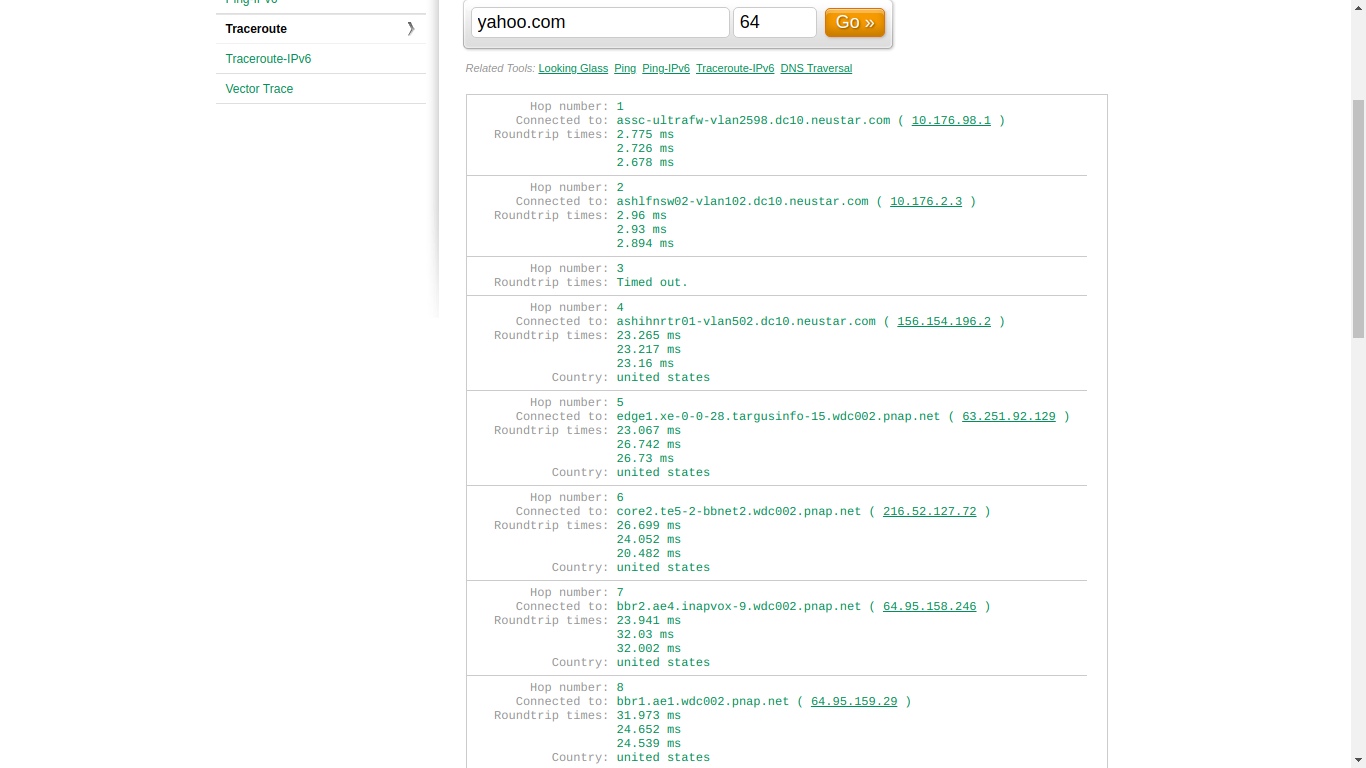
\includegraphics[width=1.0\textwidth]{Assign3/q2/q2a.png}
 \caption{\label{fig:PING}Screenshot of tcpdump file}
 \end{figure}
 
  \begin{figure}[H]
 \centering
 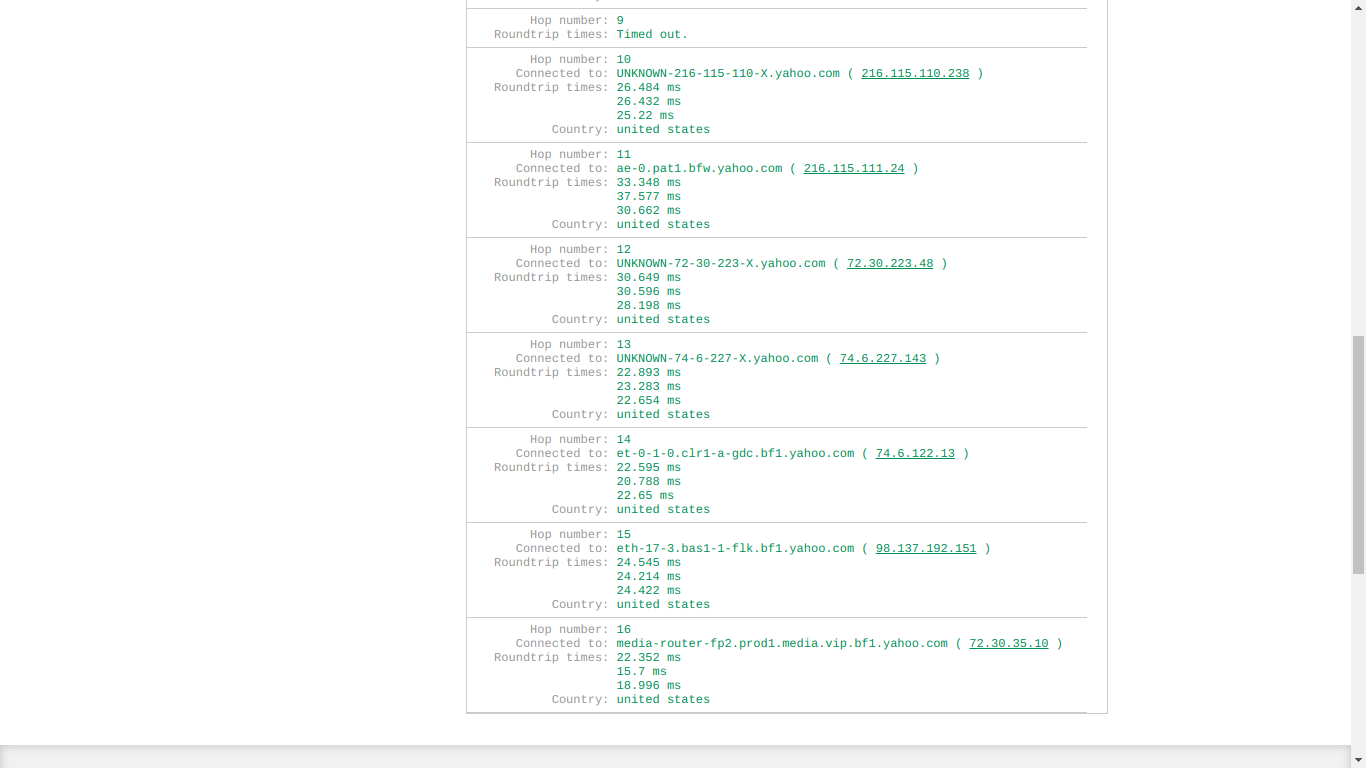
\includegraphics[width=1.0\textwidth]{Assign3/q2/q2b.png}
 \caption{\label{fig:PING}Screenshot of tcpdump file}
 \end{figure}

IP Yahoo : 72.30.35.10 \\
\\
Average round trip of packet that reached yahoo server : (22.352 + 15.7 + 18.996)/3 = 19.016
\section{Q3: output of tcpdump on TraceRoute}
\subsection{A}
3 packets are send as prooved \\
  \begin{figure}[H]
 \centering
 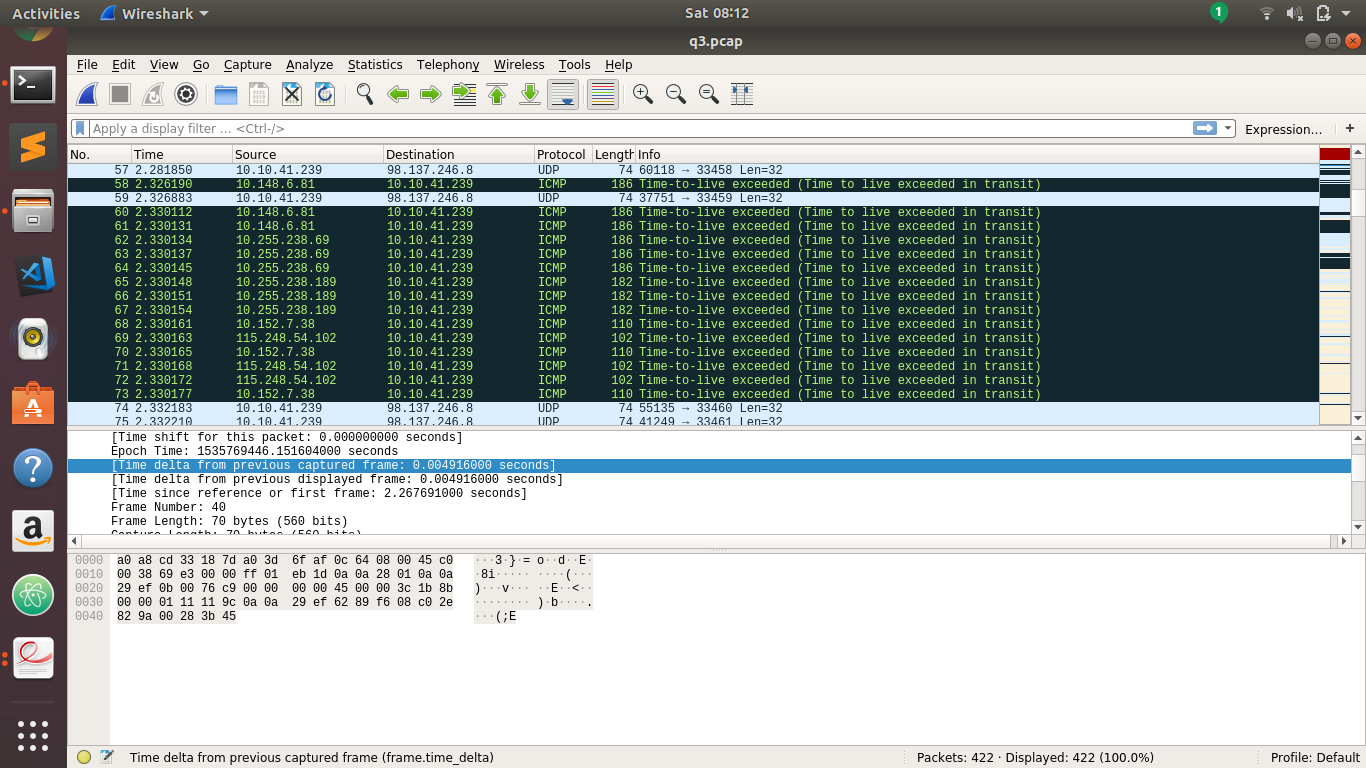
\includegraphics[width=1.0\textwidth]{Assign3/q3/q31wireshark.png}
 \caption{\label{fig:PING}Screenshot of tcpdump file}
 \end{figure}
   
   \begin{figure}[H]
 \centering
 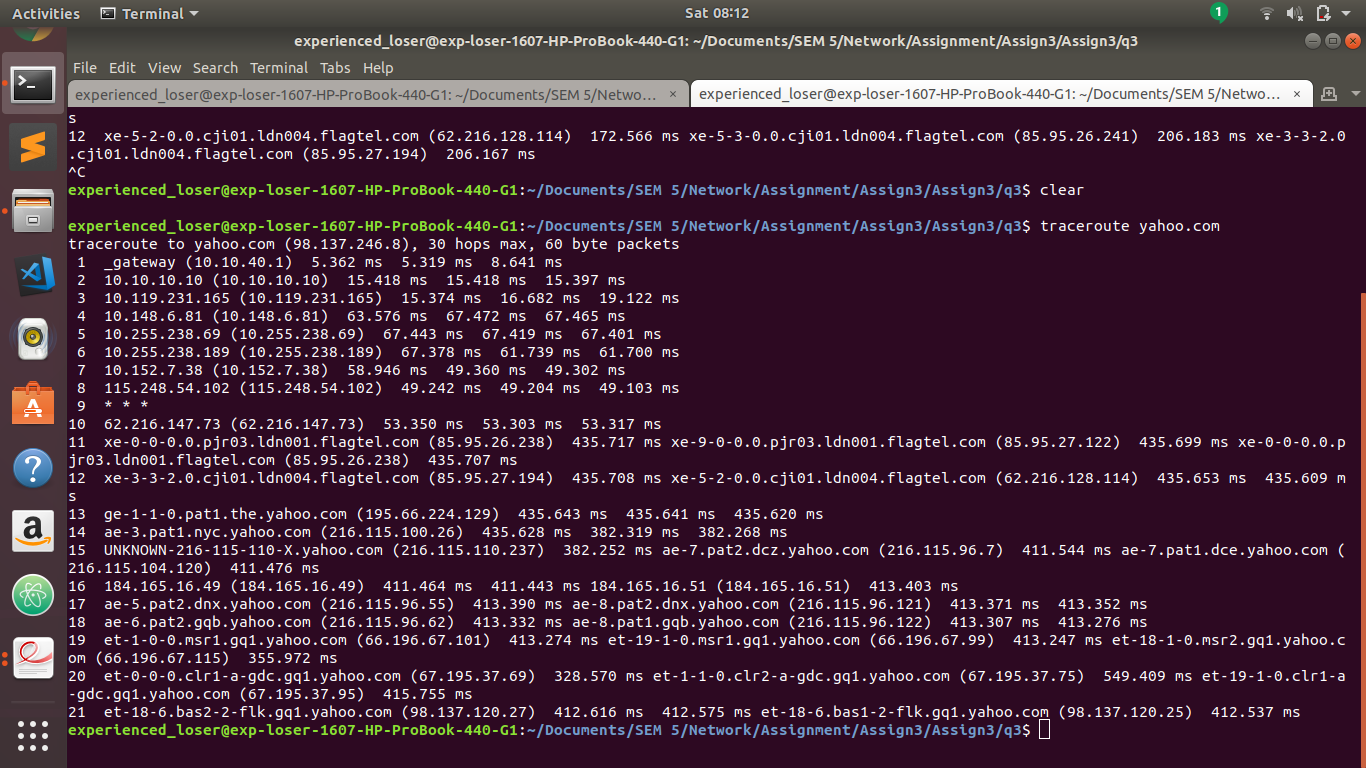
\includegraphics[width=1.0\textwidth]{Assign3/q3/q31terminal.png}
 \caption{\label{fig:PING}Screenshot of tcpdump file}
 \end{figure}
 
\subsection{B}
   \begin{figure}[H]
 \centering
 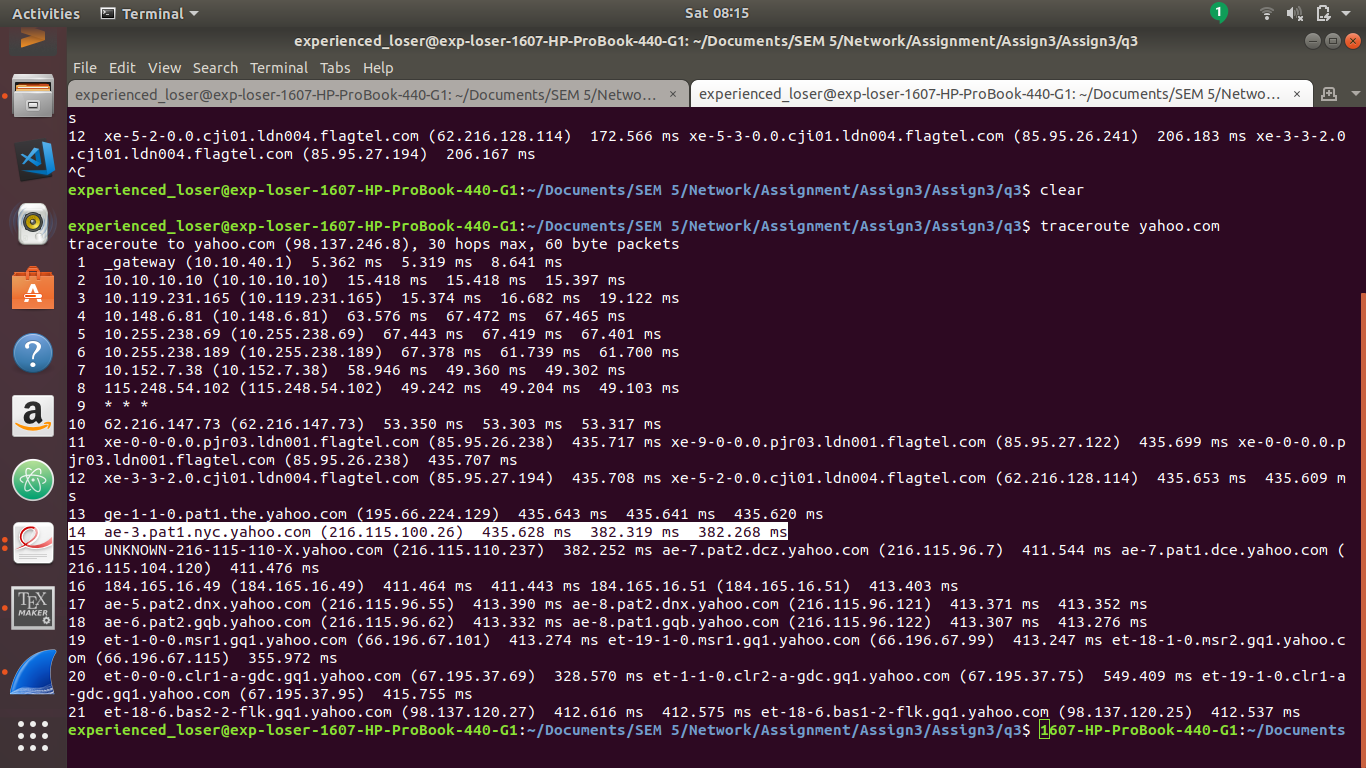
\includegraphics[width=1.0\textwidth]{Assign3/q3/q32.png}
 \caption{\label{fig:PING}Screenshot of tcpdump file}
 \end{figure}
    
    \begin{figure}[H]
 \centering
 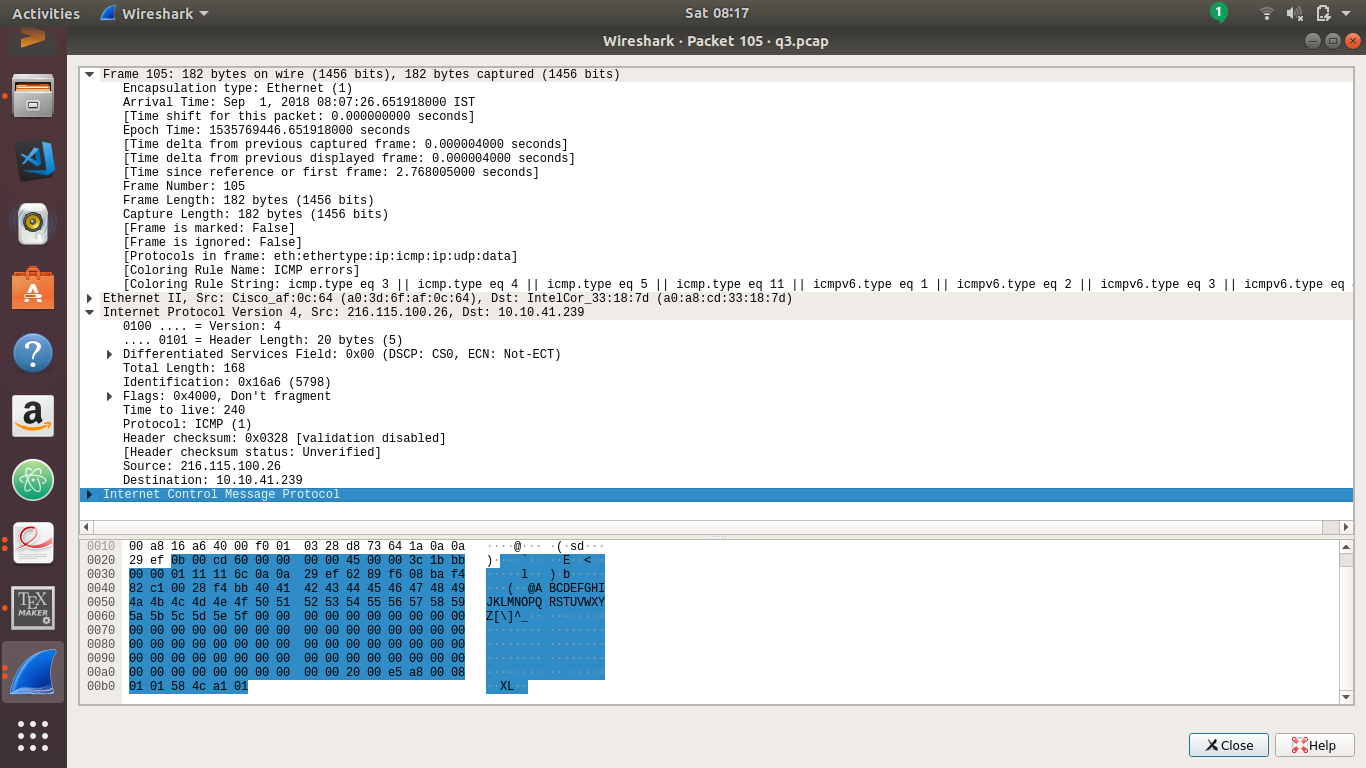
\includegraphics[width=1.0\textwidth]{Assign3/q3/q32a.png}
 \caption{\label{fig:PING}Screenshot of tcpdump file}
 \end{figure}
 
    \begin{figure}[H]
 \centering
 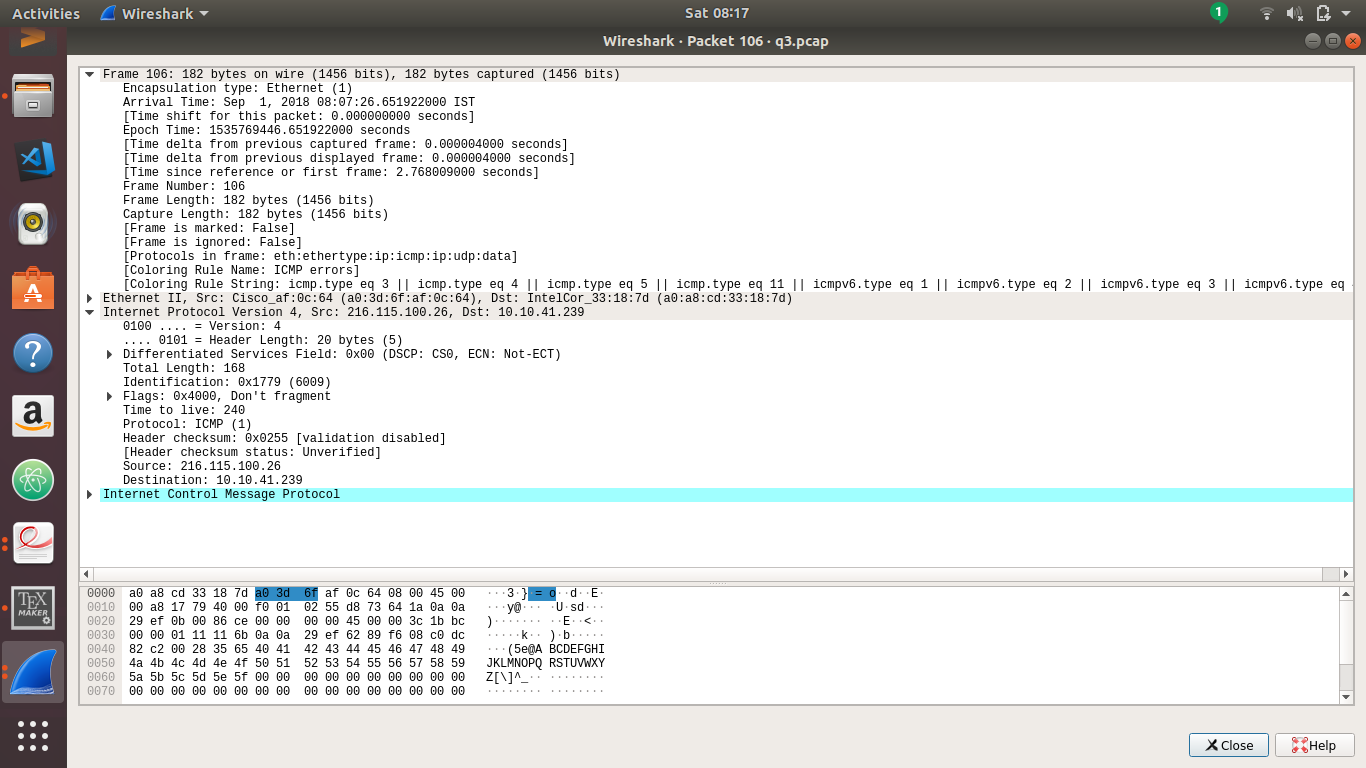
\includegraphics[width=1.0\textwidth]{Assign3/q3/q32b.png}
 \caption{\label{fig:PING}Screenshot of tcpdump file}
 \end{figure}
 
    \begin{figure}[H]
 \centering
 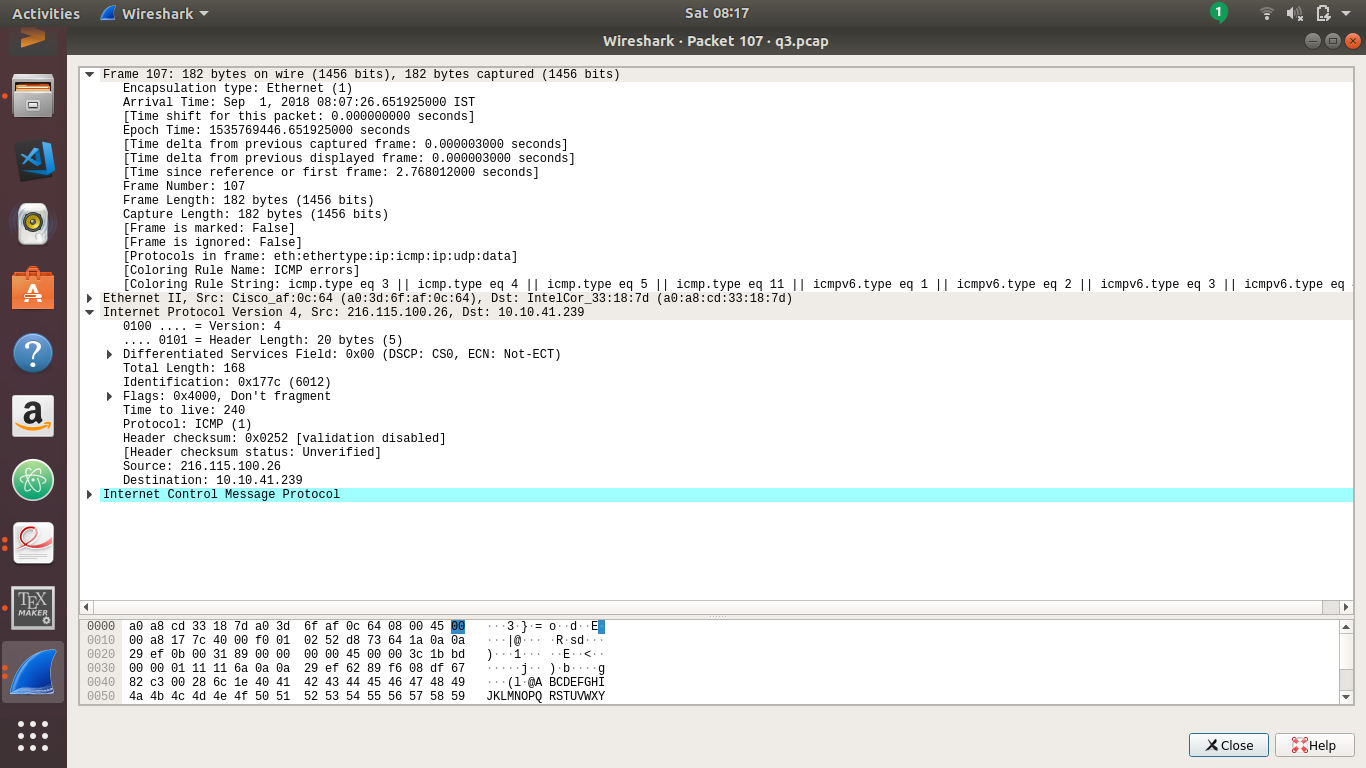
\includegraphics[width=1.0\textwidth]{Assign3/q3/q32c.png}
 \caption{\label{fig:PING}Screenshot of tcpdump file}
 \end{figure}
 
 The incidual round trip package are 435.628 , 382.319 and 382.268 .The time is not comparable from tcpdump as it gives time in contest of next frame.
\subsection{C}

  \begin{figure}[H]
 \centering
 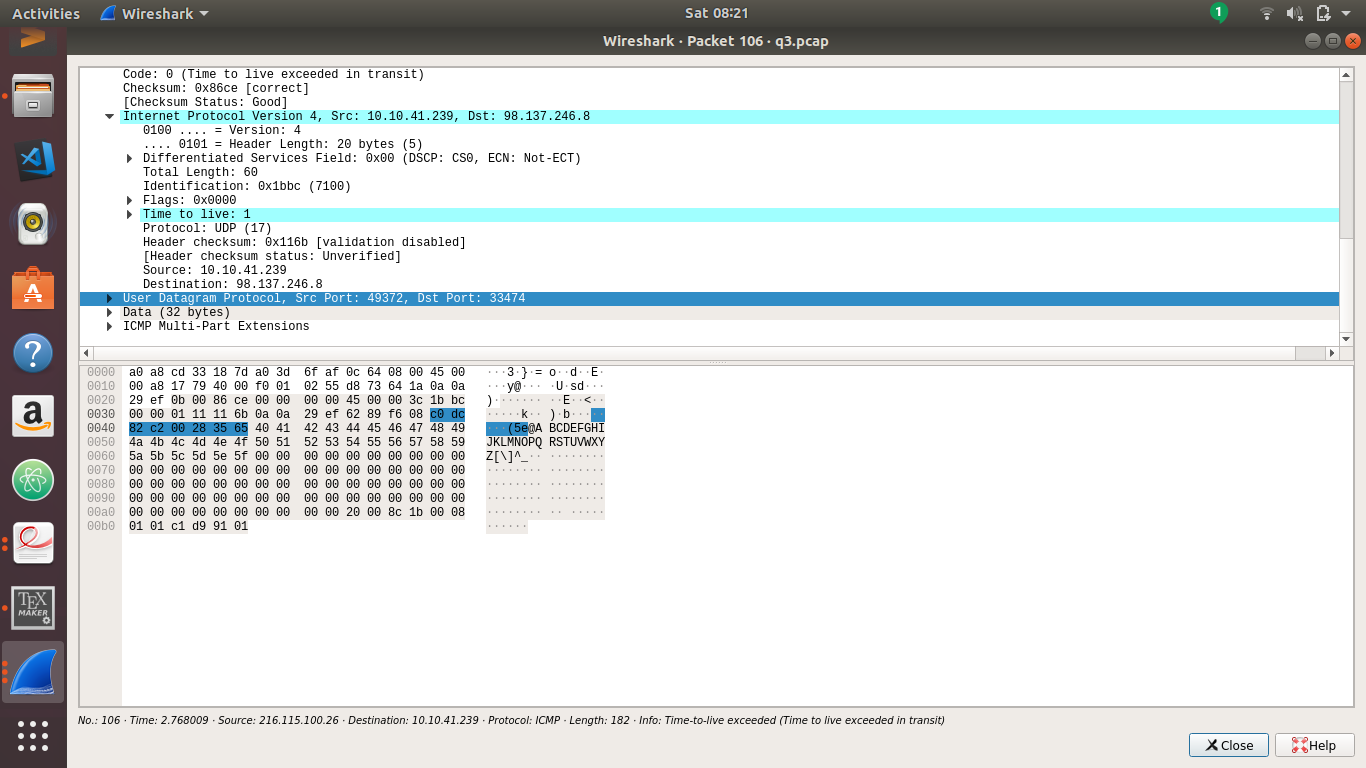
\includegraphics[width=1.0\textwidth]{Assign3/q3/q33a.png}
 \caption{\label{fig:PING}Screenshot of tcpdump file}
 \end{figure}
 
  \begin{figure}[H]
 \centering
 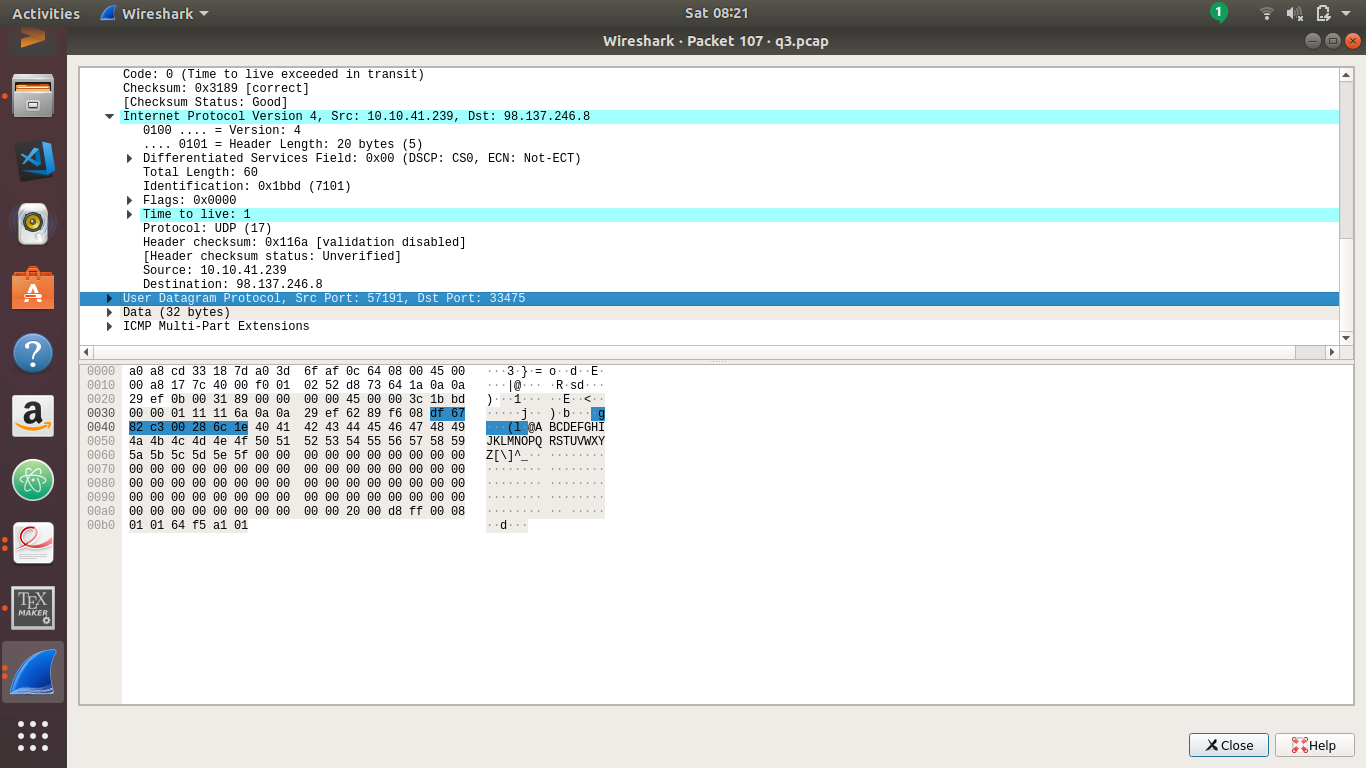
\includegraphics[width=1.0\textwidth]{Assign3/q3/q33b.png}
 \caption{\label{fig:PING}Screenshot of tcpdump file}
 \end{figure}
 No , the ports number used are different .This is so to capture icmp replies uniquely and efficiently.
\section{Q4: Visual traceroute command}
  \begin{figure}[H]
 \centering
 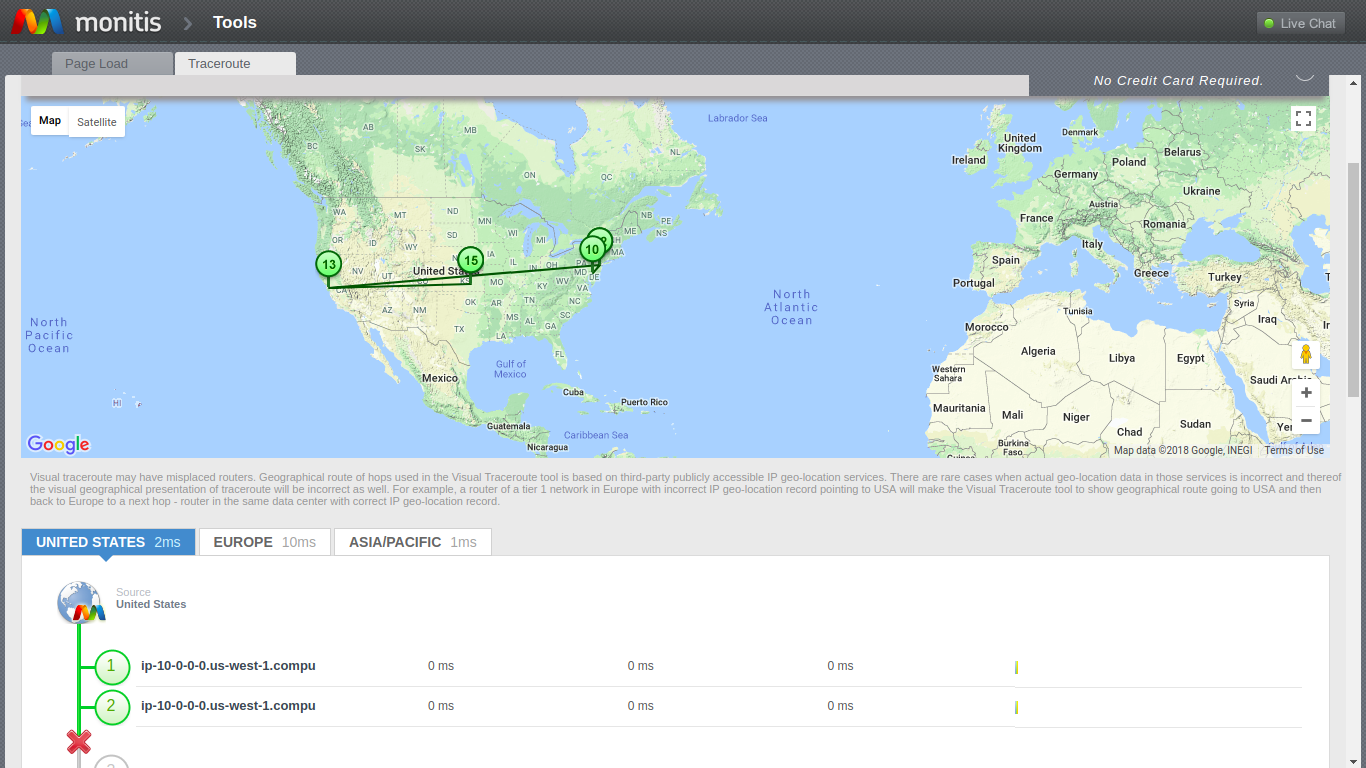
\includegraphics[width=1.0\textwidth]{Assign3/q4/q4a.png}
 \caption{\label{fig:PING}Screenshot of tcpdump file}
 \end{figure}
 
   \begin{figure}[H]
 \centering
 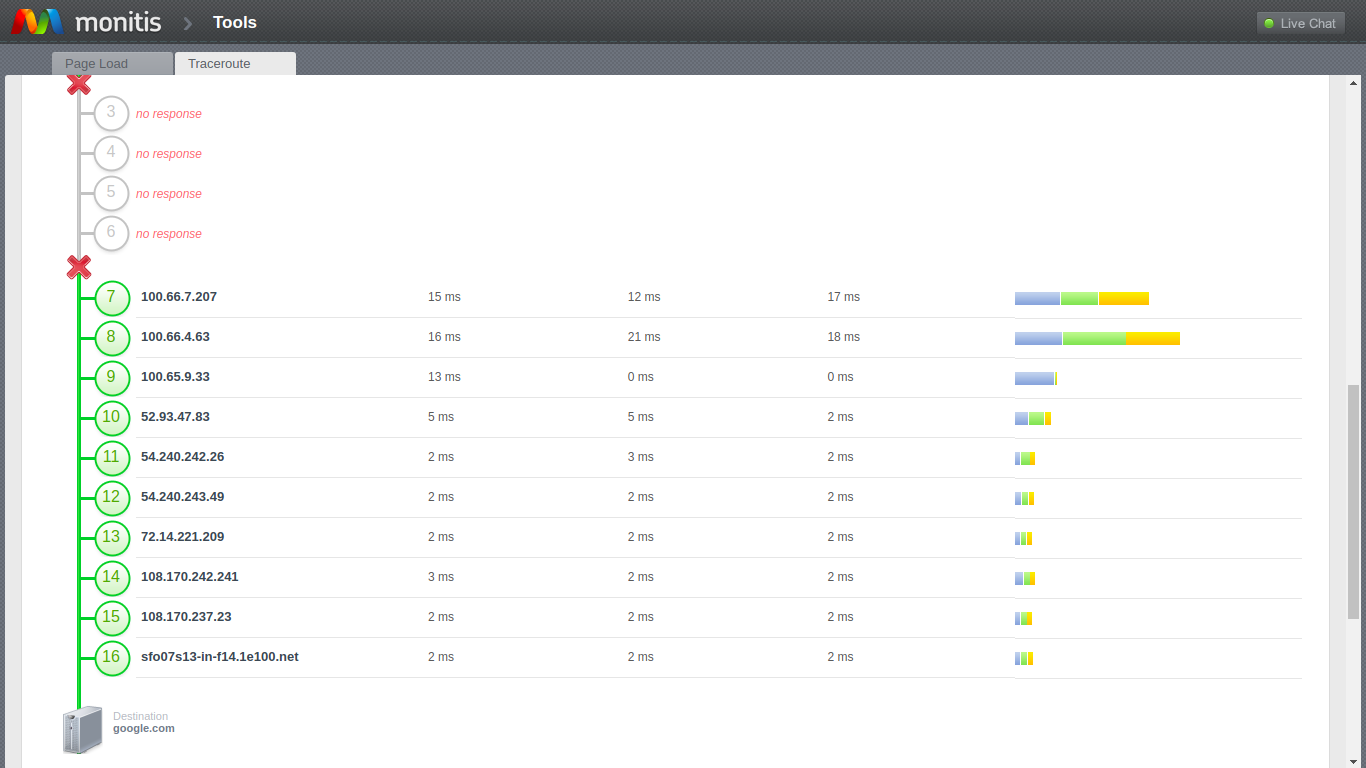
\includegraphics[width=1.0\textwidth]{Assign3/q4/q4b.png}
 \caption{\label{fig:PING}Screenshot of tcpdump file}
 \end{figure}

SRC: 10.0.0.0
DEST : 216.58.194.174

 
\section{Q5: firewall in the way}
If their is the firewall then the firewall may not allow all the UDP packets bypass it.Hence we will not be able to know the ip's of all routers or server beyond the firefall.Hence the last IP Displayed will be the ip of the firewall.

\section{Q6: last IP address in traceRoute list indicate}
If firewall allows the packet to pass then the last IP is the ip of the destination .

\section{Q7: ping program}
Ping Command Examples

\textbf{ping -n 5 -l 1500 www.google.com}
In this example, the ping command is used to ping the hostname www.google.com.\\
The -n option tells the ping command to send 5 ICMP Echo Requests instead of the default of 4, and the -l option sets the packet size for each request to 1500 bytes instead of the default of 32 bytes.\\

The result displayed in the Command Prompt window will look something like this:\\

Pinging www.google.com [74.125.224.82] with 1500 bytes of data:\\
Reply from 74.125.224.82: bytes=1500 time=68ms TTL=52\\
Reply from 74.125.224.82: bytes=1500 time=68ms TTL=52\\
Reply from 74.125.224.82: bytes=1500 time=65ms TTL=52\\
Reply from 74.125.224.82: bytes=1500 time=66ms TTL=52\\
Reply from 74.125.224.82: bytes=1500 time=70ms TTL=52\\
Ping statistics for 74.125.224.82:\\
   Packets: Sent = 5, Received = 5, Lost = 0 (0% loss),\\
Approximate round trip times in milli-seconds:\\
   Minimum = 65ms, Maximum = 70ms, Average = 67ms\\
The 0 loss reported under Ping statistics for 74.125.224.82 tells me that each ICMP Echo Request message sent to www.google.com was returned. This means that, as far as this network connection goes, it can communicate with Google's website just fine.\\

\textbf{ping 127.0.0.1}
In the above example, we're pinging 127.0.0.1, also called the IPv4 localhost IP address or IPv4 loopback IP address, without options.\\

Using the ping command to ping 127.0.0.1 is an excellent way to test that Windows' network features are working properly but it says nothing about your own network hardware or your connection to any other computer or device. The IPv6 version of this test would be ping ::1.\\

\textbf{ping -a 192.168.1.22}
In this example, we're asking the ping command to find the hostname assigned to the 192.168.1.22 IP address, but to otherwise ping it as normal.\\

Pinging J3RTY22 [192.168.1.22] with 32 bytes of data:\\
Reply from 192.168.1.22: bytes=32 time\\
As you can see, the ping command resolved the IP address we entered, 192.168.1.22, as the hostname J3RTY22, and then executed the remainder of the ping with default settings.\\

\textbf{ping 192.168.2.1}
Similar to the ping command examples above, this one is used to see if your computer can reach your router. The only difference here is that instead of using a ping command switch or pinging the localhost, we're checking the connection between the computer and the router (192.168.2.1 in this case).\\

If you're having troubles logging in to your router or accessing the internet at all, see if your router is accessible with this ping command, of course, replacing 192.168.2.1 with your router's IP address.\\

\textbf{ping -t -6 SERVER}
In this example, we force the ping command to use IPv6 with the -6 option and continue to ping SERVER indefinitely with the -t option.\\

Pinging SERVER [fe80::fd1a:3327:2937:7df310] with 32 bytes of data:\\
Reply from fe80::fd1a:3327:2937:7df310: time=1ms\\
Reply from fe80::fd1a:3327:2937:7df310: time\\
We interrupted the ping manually with Ctrl+C after seven replies. Also, as you can see, the -6 option produced IPv6 addresses.
\section{Q8: shell script that uses ping to simulate the working of traceroute}
    \begin{figure}[H]
 \centering
 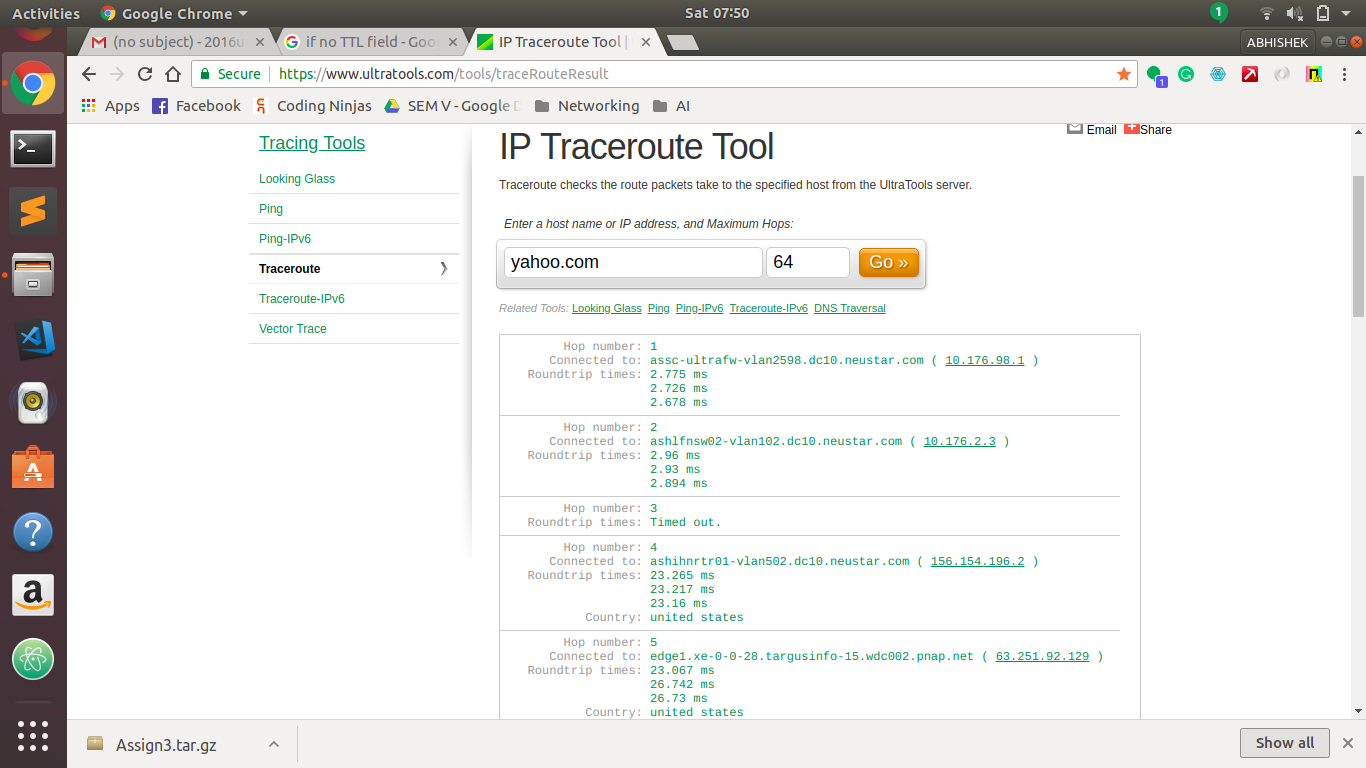
\includegraphics[width=1.0\textwidth]{Assign3/q8/q8a.png}
 \caption{\label{fig:PING}Screenshot of tcpdump file}
 \end{figure}
 
    \begin{figure}[H]
 \centering
 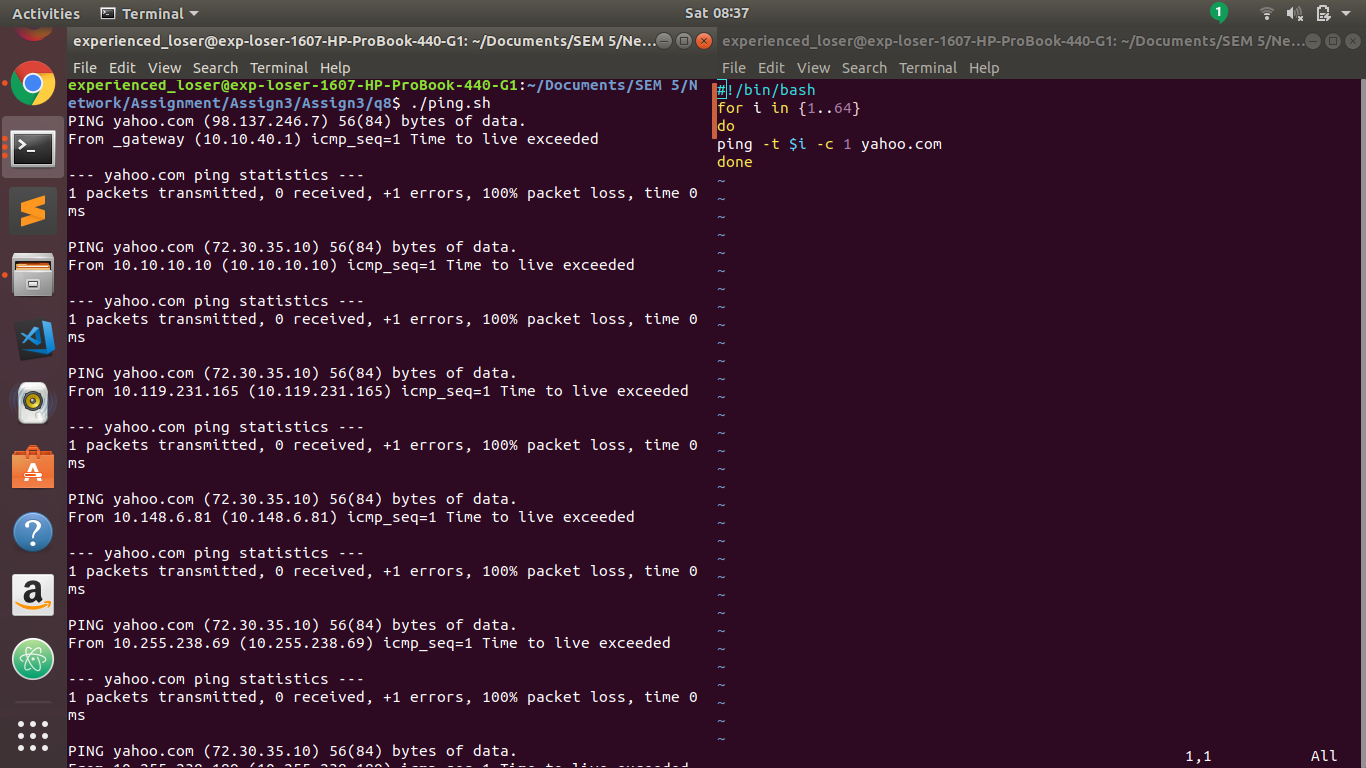
\includegraphics[width=1.0\textwidth]{Assign3/q8/q8b.png}
 \caption{\label{fig:PING}Screenshot of tcpdump file}
 \end{figure}
 ping operations \\
 -t: ttl ping only.  Set the IP Time to Live.\\
 -c: Stop  after  sending  count  ECHOREQUEST packets. With deadline option, ping waits        for count ECHOREPLY packets, until the timeout expires.\\
 1 : to try only once
\section{Q9: ping sweep}
Ping sweep is the process of pinging an entire range of network ip addresses to find out which ones are online or alive\\
There are many ways to ping sweeping. Many of them are as follows :-
\subsection{NMAP}
\textbf{nmap -sP 192.168.1.1-255}
The above command scanned all ip addresses from 192.168.1.1 to 192.168.1.255 and found out 5 ips online. The command was run on linux without root privileges.
\subsection{fping}
Normal ping command, only sends ICMP echo request to a single IP or host, at a time. However fping can be used to send ICMP echo request to a large number of hosts. It does not work like ping, because it sends an echo request to a host, and move on to the next host, not waiting for the echo reply. This is done in a round robin fashion.
\subsection{Tcp Ping Scan}
Ping Sweeping A network Which has blocked ICMP. ... So in such cases nmap tool has a good option to determine which hosts are alive in the network. For achieving this, nmap uses TCP to scan the network instead of ICMP. It is called as tcp ping scan. The command for this is ” nmap -sP -PT80 192.168.0.1-30
”.
\subsection{Simple Bash Loop}
Described above in question 8

\end{document}